\documentclass[a4paper]{article}
\usepackage[polish]{babel}
\usepackage[cp1250]{inputenc}
\usepackage[T1]{fontenc}
\usepackage[dvips]{graphicx}

\pagestyle{headings}
\textwidth      15.5cm
\oddsidemargin    .1cm
\evensidemargin   .1cm

\begin{document}

\thispagestyle{empty}

\begin{minipage}{5cm}
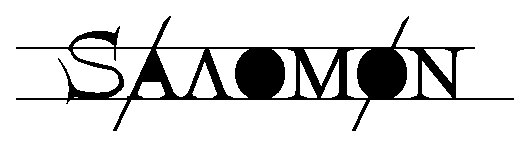
\includegraphics[scale=0.7]{salomon.eps}
\end{minipage}
\begin{minipage}{10cm}
\begin{center}
{\Large Salomon\\
System przetwarzania wiedzy\\}
\end{center}
\end{minipage}

\vspace*{0.5cm}

\hrulefill

\vspace*{1cm}


\begin{flushright}
{\Large \emph{Iteration Description --- C2, ver 1.0} }
\end{flushright}



\begin{flushleft}
{ \Large Historia wersji }\[\]
\begin{tabular}{|p{2.5cm}||p{1.5cm}|p{6cm}|p{3.5cm}|}
  \hline
  Data & Wersja & Opis & Autor \\
  \hline \hline
  29.09.2005 & 1.0 & utworzenie & \emph{Leszek Grzanka}\\
  \hline
  \hline
\end{tabular}
\end{flushleft}

\newpage

\section{Zadania dla iteracji } 
Pe�na implementacja warstwy Solution, obejmuj�ca rozbudow� GUI o mo�liwo�� pracy i zarz�dzania t� warstw�. Dodatkowo konieczne jest rozbudowanie GUI o elementy zarz�dzaj�ce pozosta�ymi warstwami: Projektami, Wtyczkami i Zadaniami.

\section{Produkt iteracji} 
Graficzny interfejs u�ytkownika pozwalaj�cy na wygodn� prac� z wszystkimi warstwami obecnymi w platformie Salomon.

\section{Plan test�w} 
\begin{itemize}
\item testowanie GUI
\end{itemize}

\section{Efekt wykonania iteracji}
W efekcie wykonania tej fazy GUI wzbogaci�o si� o kilka nowych menu i ramek umo�liwiaj�cych standardowe operacje na warstwach w platformie Salomon - dodawanie, edycja, usuwanie, otwieranie. Dodana zosta�a tak�e mo�liwo�� przegl�dania obiekt�w poszczeg�lnych warstw, wraz z mo�liwo�ci� wyszukiwania. Dodatkowo u�ytkownik ma mo�liwo�� pracy w konsoli SQL, oraz podgl�dania raport�w platformy w odpowiednim pasku statusu.


\end{document}

